\documentclass[11pt,a4paper]{article}
\usepackage{{../../paquete-formulas}}
\usepackage{{../../estilos-formulas}}


\newcommand{\materia}{Máquinas Térmicas}
\newcommand{\vs}{\vspace{-.3cm}}


\begin{document}
	\pagestyle{pieyencabezado}
	
	\section*{Nomenclatura}
	\begin{tabular}{r l}
		PCI [kcal/kg$_{comb}$] & Poder calorífico inferior \\
		PCS [kcal/kg$_{comb}$] & Poder calorífico superior \\
		H, S, C, O & \% del elemento en peso por kilogramo de combustible (cant. centesimal)\\
		H$_2$O & \% de humedad en el combustible \\
		G & Peso\\
		m & Masa\\
		C & Calor latente\\
		c$_p$ & Calor específico
	\end{tabular}

	\unidad{2}{Combustibles para generadores de calor}
	
	\begin{multicols}{2}
		\begin{cajita}
			
			\subtitulo{Poder calorífico}
			
			\vspace{.2cm}
			
			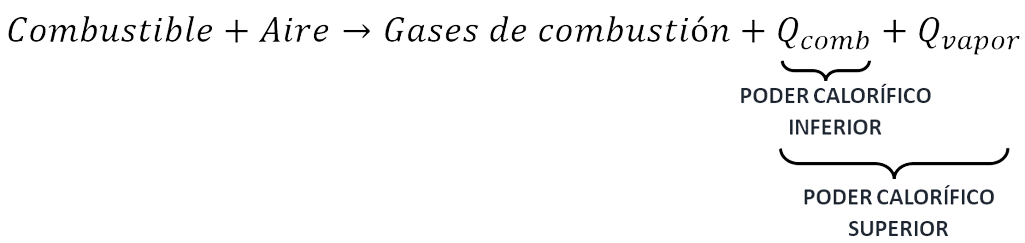
\includegraphics[width = \linewidth]{U2-poderes-calorificos}\vs
			
			\begin{flushleft}
				Relación entre los poderes caloríficos
			\end{flushleft}\vspace{-.2cm}
			
			$PCI = PCS - Q_{vapor} = PCS - 579 G$\vspace{.2cm}
			
			
			\boxed{PCI = PCS - 579 \left(9H+H_2O\right)}\vspace{.2cm}
			
			\begin{tabular}{r p{.7\linewidth}}
				$Q_{vapor}$ & Calor de condensación del vapor de agua\\
				$G$ & \% en peso del agua formada por la combustión más la humedad del combustible.\\
				$597$ & Calor de condensación del agua a $0^\circ C$.
			\end{tabular}
			
			\subsubtitulo{Hidrógeno}
			\vspace{-.8cm}
			
			
			\begin{flushleft}
				Reacción química de la combustión completa del hidrógeno
			\end{flushleft}\vs
			
			$H_2 + \frac{1}{2}O_2 \rightarrow H_2O + \boxed{34400} \left[\frac{kcal}{kg_H}\right]$
		
		\subsubtitulo{Carbono}
		\vspace{-.8cm}
		
		\begin{flushleft}
			Reacción química de la combustión completa del carbono
		\end{flushleft}\vs
	
		$C + O_2 \rightarrow CO_2 + \boxed{8140} \left[\frac{kcal}{kg_C}\right]$
		
		\begin{flushleft}
			Reacción química de la combustión incompleta del carbono
		\end{flushleft}\vs
	
		$C + \frac{1}{2} O_2 \rightarrow CO + \boxed{2440} \left[\frac{kcal}{kg_C}\right]$
			
		\subsubtitulo{Azufre}
		\vspace{-.8cm}
		
		\begin{flushleft}
			Reacción química de la combustión para el azufre.
		\end{flushleft}\vs
	
		$S + O_2 \rightarrow SO_2 + \boxed{2220} \left[\frac{kcal}{kg_S}\right] $
		
		\end{cajita}
		\columnbreak
		\begin{cajita}
			\subtitulo{Método analítico}
			
			\subsubtitulo{Fórmula de Dulong}
			\vspace{-.8cm}
			
			\begin{flushleft}
				PC de un combustible seco
			\end{flushleft}
			
			\vspace{-.2cm}
		
			\boxed{PCS = PCI = 8140  C + 34400 \left(H - \dfrac{O}{8} \right) + 2220 S}
			
			\begin{flushleft}
				PCI de un combustible húmedo
			\end{flushleft}
			
			\vspace{-.2cm}
			
			\boxed{PCI = 8140  C + 34400 \left(H - \dfrac{O}{8} \right) + 2220 S - 600 H_2O}
			
			\subsubtitulo{Fórmula de Hutte}
			
			\vspace{-.8cm}
			
			\begin{flushleft}
				PCS de un combustible húmedo
			\end{flushleft}
		
			\vspace{-.2cm}
			
			\boxed{PCI = 8100  C + 29000 \left(H - \dfrac{O}{8} \right) + 2500 S - 600 H_2O}
			
			\subsubtitulo{Fórmula de la Asociación de Ingenieros Alemanes}
			
			\vspace{-.8cm}
			
			\begin{flushleft}
				PCI de un combustible húmedo
			\end{flushleft}
			
			\vspace{-.2cm}
			
			\boxed{PCI = 8080  C + 29000 \left(H - \dfrac{O}{8} \right) + 2500 S - 600 H_2O}
			\vspace{.2cm}
			
			\begin{tabular}{r p{.7\linewidth}}
				$\dfrac{O}{8}$ & \% de $H_2$ en peso combinado con el $O_2$ del combustible dando \emph{agua de combinación}\\
				$H - \dfrac{O}{8}$ & \% de \emph{hidrógeno disponible} en peso que se oxida con el aire ($O_2$) para dar \emph{agua de formación}
			\end{tabular}
		\end{cajita}
	\end{multicols}
	
	\begin{cajita}
		
		\subtitulo{Método práctico}
		
		\subsubtitulo{Calorímetro de Mahler y Kroeker}\vspace{-.6cm}
		
		\begin{multicols}{2}
			\begin{flushleft}
				Supone que el calor $Q$ generado dentro de la bomba calorimétrica es absorbido por los elementos que la rodean:
				\begin{itemize}
					\item Agua contenida\\[.1cm]
					\item Agitador\\[.1cm]
					\item Termómetro\\[.1cm]
					\item Bomba\\[.1cm]
					\item Recipiente
				\end{itemize} 
			
				Y dicho calor es cedido por la combustión y el alambre:
			\end{flushleft} 
			\begin{tabular}{r c l}
				$Q$ & = & $Q_{combustible} + Q_{alambre}$\\[.2cm]
					& = & $\left(m_{w} {c_p}_{w} + E_{aparato}\right) \Delta t$\\[.2cm]
			\end{tabular}
			
			
			
			$PCS = \dfrac{Q_{comb}}{G_{comb}}$\\[.1cm]
			
				\columnbreak
			
			\boxed{PCS = \dfrac{\left(m_{w} {c_p}_{w} + E_{aparato}\right) \Delta t - m_{alam} C_{alam}}{G_{comb}}}\\[.1cm]
			\boxed{PCI = PCS - 600 \dfrac{G_w}{G_{comb}}}
			\vspace{.3cm}
		
			
			\begin{tabular}{r p{.7\linewidth}}
				$G_w$ & Peso total de agua existente $= papel\,húmedo - papel\, seco$\\
				$G_{comb}$ & Peso de combustible quemado\\
			\end{tabular}
		\end{multicols}
		
	\end{cajita}
	
	\begin{cajita}
			\begin{center}
				\begin{tabular}{r l}
					Relación entre los poderes caloríficos: & \boxed{PCI = PCS - 597 \times G= PCS - 597(9H+H_{2}O)}\\
				\end{tabular}
			\end{center}
			\begin{multicols}{2}
			Siendo:\\
				\begin{tabular}{r p{0.4\textwidth}}
					597	& Calor de condensación del agua a O ºC \\
					G & Porcentaje en peso del agua formada por la combustión del $H_{2}$ más la humedad propia del combustible\\
				\end{tabular}
			\newpage
			
			Recordando: \boxed{G=9H+H_{2}O} $\uparrow$\\
			
				\begin{tabular}{r p{0.4\textwidth}}
					9 & Son los kilos de agua que se forman al oxidar un kilo de  hidrógeno.\\
					H & \% de hidrógeno contenido en el combustible.\\
					H2O & \% de humedad del combustible.\\
				\end{tabular}
			\end{multicols}
		
	\begin{center}
		\subtitulo{ Método analítico}
	\end{center}
%\vspace{0.2cm}
	\begin{tabular}{l l}
		\multicolumn{2}{l}{\textbf{Formulas de Dulong}}\\
		PCS comb. seco & \boxed{PCS	=	8.140  \times	C	+ 34.400	\times	(H -	O/8)	+	2.220	\times	S}\\
		PCI comb. seco: &\boxed{PCI = 8.140 \times C + 29.000 \times (H - O/ 8 ) + 2.220 \times S}\\
		PCI comb. húmedo:&\boxed{PCI = 8.140 \times C + 29.000 \times (H - O/ 8 ) +  2.220 \times S - 600 \times H2O}\\[0.2cm]
		\multicolumn{2}{l}{\textbf{Formula de Hutte}}\\
		PCI comb. húmedo & \boxed{8.100 \times C + 29.000 \times (H - O/ 8 ) + 2.500 \times S -  600 \times H2O}\\[0.2cm]
		\multicolumn{2}{l}{\textbf{Formula de Asociación de Ing. Alemanes}}\\
		PCI comb. húmedo& \boxed{PCI = 8.080 \times C + 29.000 \times (H - O/ 8 ) + 2.500 \times S -  600 \times H2O}\\
	\end{tabular}
	\begin{flushleft}
		\begin{tabular}{r p{0.87\textwidth}}
				C & Cantidad centesimal de carbono en peso por kilogramo combustible\\
				H & Cantidad centesimal de hidrógeno total en peso por kilogramo de
				combustible\\
				O & Cantidad centesimal de oxígeno en peso por kilogramo combustible\\
				S & Cantidad centesimal de azufre en peso por kilogramo combustible\\
				O / 8 & Cantidad centesimal de hidrógeno en peso que se encuentra combinado con el oxígeno del mismo combustible dando ``agua de  combinación''\\
				(H - O/8 ) &  Cantidad centesimal de ``hidrógeno disponible'', en peso  realmente disponible para que se oxide con el oxígeno del aire,  dando ``agua de formación''\\
			\end{tabular}
		\end{flushleft}

	\begin{center}
		\subtitulo{ Método práctico}		
	\end{center}
		CALORIMETRO DE MAHLER Y KROEKER
			\begin{flushleft}
			\begin{tabular}{r p{0.85\textwidth}}
				$Q$=&$Q_{agua}+Q_{termometro}+Q_{agitador}+Q_{recipiente}+Q_{vaso}$\\
				$Q$=&$\Delta T (m_{agua}~cp_{agua}+m_{termometro}~cp_{termometro}+m_{agitador}+cp_{agitador}+m_{recipiente}~cp_{recipiente}+m_{vaso}~cp_{vaso})$\\
				$Q$&$\left(m_{agua}~cp_{agua}+E_{aparato}\right)\Delta T$\\					
				\multicolumn{2}{l}{	Para determinar el poder calorifico:}\\
				$Q$=&$Q_{combustible}+Q_{alambre}$\\
				$Q_{comb}$=&$Q-Q_{alambre}$\\
				\multicolumn{2}{l}{Reemplazo:}\\
				$Q_{comb}$=&$\left(m_{agua}~cp_{agua}+E_{aparato}\right)\Delta T - m_{alambre} ~ C_{alambre}$ \\
				\multicolumn{2}{l}{Nos queda:}\\
				PCS=&$\dfrac{Q_{combustible}}{G_{combustible}}$\\
				PCI=& $PCS-600	( 9H	+ H2O )$=$ PCS	-	600	\dfrac{G_{agua}}{G_{combustible}}$\\
			\end{tabular}\\
		\textit{$G_{agua}$ representa el peso del total de agua existente = (peso papel humedo - peso papel seco)\\
			    $G_{combustible}$ el peso de combustible quemado}
		\end{flushleft}
	
		\section*{Aire mínimo para una combustión perfecta}
		\begin{equation}
			G_{t \ aire} = 11.6 g_{c} + 34.78 g_{hd} +4.35 g_{s} \; [Kg_{aire}/Kg_{comb.}]
		\end{equation}
		\begin{equation}
			V_{t \ aire} = 8.89 g_{c} + 26.27 g_{hd} + 3.34 g_{s} \; [m^{3}_{aire}/Kg_{comb.}]
		\end{equation}
		\begin{flushleft}
			Donde 
		
		$g_{hd} = g_{h} - \dfrac{g_{o_{2}}}{2}$
		
		$g_{c}$ composición gravimétrica carbono
		
		$g_{h}$ composición gravimétrica hidrógeno
		
		$g_{o_{2}}$ composición gravimétrica oxígeno
		
		$g_{s}$ composición gravimétrica azufre
		
		-
		\\
	
		En la práctica es necesario trabajar con un exceso de aire para que asegurar la combustión perfecta:
		\end{flushleft}
		\begin{equation}
			V_{R \ aire} = (1+e) V_{t \ aire} [m^{3}_{aire}/Kg_{comb.}]
		\end{equation}
		
		\section*{Gases de combustón}
		\begin{equation}
			g_{h} = (3.67 g_{c} + 9 g_{hd} +2 g_{s}) + 3.35 (2.67 g_{c} + 8 g_{hd} + g_{s}) + g_{w} \; [Kg_{humo}/Kg_{comb}]
		\end{equation}
		\begin{equation}
			V_{h} = 1.897 g_{c} + 11.2 g_{hd} +0.7 g_{s} + 3.76 (1.867 g_{c} + 5.6 g_{hd} +0.7 g_{s}) + 1.24 g_{w} \; [m^{2}_{humo}/Kg_{comb}]
		\end{equation}
	\end{cajita}
	
	\begin{cajita}
		\subtitulo{Exceso de aire}
%		\begin{flushleft}
%			$g_{h}\left(\dfrac{\textnormal{Kg gases húmedos}}{\textnormal{Kg de combustible}}\right) = 1 \left(\dfrac{\textnormal{Kg producto}}{\textnormal{Kg de combustible}}\right) + e~G_{AT} \left(\dfrac{\textnormal{Kg de aire teórico}}{\textnormal{Kg de combustible}}\right)$\\
%			$e= \dfrac{g_{h}-1}{G_{AT}}$
%		\end{flushleft}
		\begin{multicols}{2}
			\begin{tabular}{r p{0.87\textwidth}}
				$g_{h}$ & (kg de gases húmedos/ kg de combustible)\\
				$e$ & (coeficiente de exceso de aire)\\
				$g'_{S}$ & (kg gases secos / kg carbono)\\
				$g''_{S}$ & (kg gases secos / kmol combustible)\\
				$\mu$ & (masa molecular) (kg/kmol)\\
				$G_{AT}$ & (kg de aire teórico / kg de combustible)\\
				$g_{S}$ & (kg gases secos/ kg de combustible)\\
				$g_{C}$ & kg de carbono / kg de combustible)\\
				$g'_{C}$ & (kg carbono / kmol combustible)\\
				$g{w}$ & (kg de aire teórico/ kg combustible)\\
				$r$ & composición volumentrica\\
				
			\end{tabular}
			\begin{tabular}{r l }
			$g_{h}=$&$1+e~G_{AT}$\\[0.2cm]
			$e=$&$\dfrac{g_{h}-1}{G_{AT}}$\\
			$g_{h}=$&$g_{s}+g_{w}$\\
			$g_{S}=$&$g'_{S}~g_{C}$\\
			\end{tabular}
			\begin{tabular}{r l }
				$g'_{S}=$&$\dfrac{G''_{S}}{g'_{C}}$\\
				$g_{i}=$&$\mu_{i}~r_{i}$\\[0.3cm]
				$g''_{S}=$&$\displaystyle \sum_{i=1}^{n} \mu_{i}~r_{i}$\\[0.3cm]
				$g'_{C}=$&$\displaystyle \sum_{i=1}^{n} \mu_{C}~r_{iC}$\\[0.3cm]
				$g'_{S}=$&$\dfrac{\sum_{i=1}^{n} \mu_{i}~r_{i}}{\sum_{i=1}^{n} \mu_{C}~r_{iC}}$\\[0.3cm]
				$g_{h}=$&$\dfrac{\sum_{i=1}^{n} \mu_{i}~r_{i}}{\sum_{i=1}^{n} \mu_{C}~r_{iC}} g_{C}+g_{w}$\\[0.35cm]
				$g_{w}=$&$9~g_{he}$\\[0.1cm]
				$G_{AT}=$&$11.6~g_{C}+37.38~g_{hd}+4.35~g_{S}$\\
				&\tiny{para mi aca gs es del azufre, no gases secos/comb.}
			\end{tabular}
		\end{multicols}
	Yo copié las formulas, pero los analisis dimensionales no dan en algunos...
	\end{cajita}
		
	\begin{cajita}
		\subtitulo{Volumen humos combustión imperfecta}
	\end{cajita}
%\left(\dfrac{\textnormal{asd}}{\textnormal{asd}}\right)

\end{document}